\section{Indicators}

Indicators play a crucial role in assessing and monitoring carbon emissions in the maritime shipping industry.
They provide valuable insights into the environmental performance of vessels,
facilitate comparisons between different ships or fleets, and help track progress towards emission reduction targets.
By measuring various aspects of emissions and energy efficiency,
these indicators enable stakeholders to identify opportunities for improvement and implement effective strategies to mitigate the environmental impact of shipping operations.

In this section, we will discuss several key indicators commonly used in the monitoring and evaluation of carbon emissions in maritime shipping.
These indicators cover a range of factors, including carbon intensity, energy efficiency, fuel consumption, and cargo transport work.
Each indicator offers a unique perspective on emissions, providing researchers, policymakers, and industry stakeholders with valuable information to support decision-making and foster sustainable practices.

It is important to note that the selection and use of indicators may vary depending on the specific research objectives, data availability, and regulatory frameworks in place.
The combination of different indicators allows for a comprehensive assessment of emissions and enables a deeper understanding of the efficiency and environmental performance of shipping activities.

Below is the list of indicators discussed in this section:

\begin{enumerate}
    \item Carbon Intensity Indicator (CII)
    \item Energy Efficiency Operational Indicator (EEOI)
    \item Energy Efficiency Design Index  (EEDI)
    \item Energy Efficiency eXisting ship Index  (EEXI)
\end{enumerate}

\subsection{Carbon Intensity Indicator (CII)}

The International Maritime Organization (IMO) has introduced a new carbon intensity (CII) measure for ships, which is a more accurate way to evaluate a vessel's environmental impact than total carbon emissions.
CII is calculated using the Annual Efficiency Ratio (AER) formula, taking into account a ship's fuel consumption, CO2 emission factor, annual distance sailed, and design deadweight.

To calculate CII in the most basic form:

\begin{equation}
    \text{CII} = \frac{\text{Carbon Emission}}{\text{Distance Travelled} \times \text{Cargo Capacity}}
    \label{eq:cii}
\end{equation}


Vessels are rated A to E based on their CII results, and those with a D or E rating for three consecutive years or an E rating in one year must submit a corrective action plan.
The IMO will enforce CII regulations for all ships over 5,000 GT and require an enhanced Ship Energy Efficiency Management Plan (SEEMP) with CII-related content from January 2023.
The SEEMP must include the ship's required annual operational CII target and an implementation plan to achieve it over the next three years. \autocite{chuah2023implementation}.

\begin{figure}[h]
    \centering
    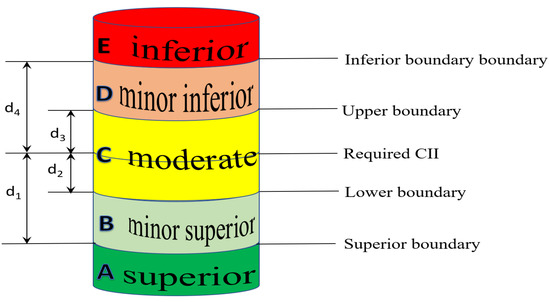
\includegraphics[width=0.5\textwidth]{images/cii_ratings.jpeg}
    \caption{Schematic diagram of the CII ratings and boundaries. \autocite{tsai2023effects}}
    \label{ciiRating}
\end{figure}


The article \cite{rodriguez2020indicators}, discusses the increasing popularity of Energy and Car- bon Intensity indicators among policy makers, which are calculated as units of energy or mass of emissions per unit of Gross Domestic Product (GDP).
These indicators are gaining momen- tum due to support from think tanks, public organizations, consulting groups, and academics focused on energy and climate change policy development.
The ways in which intensity in- dicators are framed and perceived in public debates generated by these intermediaries are important as they can influence policy making and the development of better sets of indicators to assess how well countries are addressing climate change and resource efficiency policies.
Intensity indicators are appealing for emerging economies as they are not incompatible with high rates of economic growth and do not imply the imposition of absolute emission/energy caps.


\subsection{Energy Efficiency Operational Indicator (EEOI)}

The Energy Efficiency Operational Indicator (EEOI) is a tool used to measure the CO2 gas emissions per unit of transport work, indicating the operational efficiency of a ship.
The EEOI is calculated annually and is subject to changes after each voyage due to various external factors, such as navigation conditions, sea area, weather, temperature, and cargo weight.

The EEOI provides an accurate measure for each voyage, and its unit depends on the type of cargo or transport work, such as tons CO2/(tons/nautical miles), tons CO2/(TEU/nautical miles), or tons CO2/(person/nautical miles).
The formula for calculating the EEOI is represented by formula (\ref{eq:eeoi}), where a lower value indicates a more energy-efficient ship \autocite{prill2020new}.

\begin{equation}
    \text{EEOI} = \frac{\text{Carbon Emission}}{\text{Performed Transport Work}}
    \label{eq:eeoi}
\end{equation}

For the calculation of EEOI for a specific voyage, formula (\ref{eq:eeoi_voyage}) is used.

\begin{equation}
    \text{EEOI} = \frac{\sum_{j} F_{Cj} \cdot C_{Fj}}{m_{\text{cargo}} \cdot D_j}
    \label{eq:eeoi_voyage}
\end{equation}

However, when dealing with a large number of ships, formula (\ref{eq:eeoi_voyage}) is expressed as equation (\ref{eq:eeoi_average}), taking into account parameters such as fuel type, voyage number, fuel consumption, fuel-to-CO2 conversion factor, cargo weight, and distance traveled \autocite{tran2017research}.

\begin{equation}
    \text{Average}_{\text{EEOI}} = \frac{\sum_{i}\sum_{j}(F_{C_{i}} \cdot C_{F_{j}})}{\sum_{i}(m_{\text{cargo},i} \cdot D_{i})}
    \label{eq:eeoi_average}
\end{equation}

where:
\begin{align*}
     & j: \text{Fuel type used}                                            \\
     & i: \text{Navigation voyage number}                                  \\
     & FC_{ij}: \text{Mass of consumed fuel } j \text{ at voyage } i       \\
     & CF_{j}: \text{Fuel mass to CO2 mass conversion factor with fuel } j \\
     & m_{cargo}: \text{Weight of cargo carried (tons) on ship}            \\
     & D_{i}: \text{Distance of voyage } i \text{ (nautical miles)}
\end{align*}

The fuel-to-CO2 conversion factor (CF) is a non-dimensional factor that converts fuel consumption, measured in grams, to CO2 gas emissions, also measured in grams, based on the carbon content.
The below table

\ref{tab:fuel_composition} is showed the certain value of CF follows the type of fuel.

\begin{table}[h]
    \centering
    \resizebox{\textwidth}{!}{%
        \begin{tabular}{|c|c|c|c|c|}
            \hline
            \textbf{No.} & \textbf{Type of fuel}         & \textbf{Reference}              & \textbf{Carbon content} & \textbf{CF (t-CO2/t-Fuel)} \\
            \hline
            1            & Diesel/gas oil                & ISO 8217 Grades DMX through DMC & 0.875                   & 3.206000                   \\
            \hline
            2            & Light fuel oil (LFO)          & ISO 8217 Grades RMA through RMD & 0.86                    & 3.151040                   \\
            \hline
            3            & Heavy fuel oil (HFO)          & ISO 8217 Grades RME through RMK & 0.85                    & 3.114400                   \\
            \hline
            4            & Liquefied petroleum gas (LPG) & Propane, butane                 & 0.819, 0.827            & 3.000000, 3.030000         \\
            \hline
            5            & Liquefied natural gas (LNG)   &                                 & 0.75                    & 2.750000                   \\
            \hline
        \end{tabular}
    }
    \caption{The value of CF (t-CO2/t-Fuel) \autocite{tran2017research}.}
    \label{tab:fuel_composition}
\end{table}

\subsection{Energy Efficiency Design Index  (EEDI)}


Energy Efficiency Design Index (EEDI) is a legislation proposed by the International Maritime Organization (IMO) to estimate the energy efficiency of ships and calculate their CO2 emissions per unit of transport work done during the ship design phase.
EEDI is based on a complex formula that takes into account the ship's emissions, capacity, and speed, and the lower the ship's EEDI index, the less CO2 emissions it produces.

EEDI is a non-prescriptive mechanism that allows the shipping industry to use the latest technologies for designing commercial vessels as long as they meet the required energy efficiency levels and parameters.
It lays down a minimum energy efficiency level, per capacity mile, for different ship types and sizes, including tankers, bulk carriers, gas carriers, general cargo ships, container ships, refrigerated cargo carriers, and combination carriers.

The EEDI formula has two components: attained EEDI and required EEDI.
The attained EEDI is calculated using a complex formulation based on the vessel's emissions, capacity, and speed,
while the required EEDI is the minimum level of energy efficiency that a ship must meet as per its ship type and size.
The attained EEDI is verified based on the ship's design and construction, and the required EEDI is the target that the ship must achieve during its operation \autocite{ren2019influence}.


EEDI calculation module as part of Marpol Annex VI, following the directive MEPC.1/Circ.681 at the MEPC meeting conducted by the IMO in 2011.
This regulation came into effect on January 1, 2013. The EEDI formula (Equation 1) specified by IMO (2011) is represented by the equation (\ref{eq:attained_eedi}) \autocite{tokucslu2020analyzing}.



\begin{equation}
    EEDI = \frac{{P \cdot \text{SFC} \cdot \text{Cf}}}{{DWT \cdot \text{Vref}}}
    \label{eq:attained_eedi}
\end{equation}


where:
\begin{align*}
    P              & : \text{70\% of the power of the engine (main and auxiliary) in kW}             \\
    \text{SFC}     & : \text{Amount of fuel burned by the engines in kW (specific fuel consumption)} \\
    Cf             & : \text{Emission rate of fuel used by the ship (presented in Table 1)}          \\
    DWT            & : \text{Ship's capacity (in tons)}                                              \\
    V_{\text{ref}} & : \text{Speed of the ship (in knots)}
\end{align*}


\subsection{Energy Efficiency eXisting ship Index  (EEXI)}

The Energy Efficiency Existing Ship Index (EEXI) is a regulation introduced by the International Maritime Organization (IMO) aimed at improving the energy efficiency of existing ships.
It is part of the broader effort to reduce greenhouse gas emissions from the shipping industry and combat climate change.
The EEXI is designed to complement the Energy Efficiency Design Index (EEDI), which focuses on new ship designs \autocite{czermanski2022implementation}.

The EEXI is part of a comprehensive framework that includes short-term, mid-term, and long-term measures.
The short-term measures focus on technical and operational improvements, such as retrofitting ships with energy-efficient technologies.
The mid-term measures involve market-based mechanisms to incentivize emission reductions, while the long-term measures explore alternative fuels and propulsion systems \autocite{CHUAH2023115348}.

The calculation of the Energy Efficiency Existing Ship Index (EEXI) can be optimized by considering the ship's maximum continuous rating (MCR) at 100\% capacity.
This approach ensures that improvements in technical efficiency closely align with the ship's actual operational fuel use.
By accounting for the engine power limits (EPLs) within the engine margin, which have minimal impact on ship operations, a more accurate assessment of energy efficiency can be achieved.
Currently, the proposed calculation methods for the EEXI involve using either 75\% of the limited MCR (MCRlim), similar to the Energy Efficiency Design Index (EEDI), or a higher value of 87\% MCRlim, which only considers the engine margin.
However, utilizing ship characteristics data from IHS Markit and applying the appropriate calculation method, the attained EEXI score can still be estimated, providing valuable insights into a ship's energy performance \autocite{rutherford2020potential}.

\begin{equation}
    \text{Attained EEXI} = 3.1144 \times \frac{MESFOC \times \sum_{i=1}^{nME} P_{ME,i} + AESFOC \times P_{AE}}{\text{Capacity} \times \text{Vref}}
    \label{eq:attained_eexi}
\end{equation}

The estimation of the attained EEXI score using ship characteristics data from IHS Markit, as outlined in Equation (\ref{eq:attained_eexi}), contributes to a more comprehensive understanding of a ship's energy efficiency.
This information supports decision-making processes related to optimizing operational fuel consumption, implementing retrofit measures, and promoting environmental sustainability in the maritime industry.
By calculating the EEXI at 100\% MCR, the assessment takes into account the EPLs within the engine margin, which are not expected to significantly affect ship operations.
This approach ensures that technical efficiency improvements are properly aligned with the ship's actual operational fuel use, enabling informed decision-making for enhancing operational fuel consumption and reducing environmental impact.
Through the utilization of ship characteristics data and the appropriate calculation method, the attained EEXI score serves as a valuable tool for assessing energy efficiency and driving advancements in the maritime sector \autocite{rutherford2020potential}.




